\documentclass[12pt]{article}
\usepackage[utf8]{inputenc}
\usepackage[french]{babel}
\usepackage{tikz}
\usepackage{float}
\usepackage{amsthm}
\usepackage{amssymb}
\usepackage{amsmath}
\usepackage{mathtools}
\usepackage{vmargin}
\usepackage{enumerate}
\usepackage{color,soul}
\usepackage{verbatim}
\usepackage{multirow}
\usepackage{stmaryrd}
\usepackage{fancyhdr}
\usepackage{indentfirst}

\newcommand{\hsp}{\hspace{20pt}}
\newcommand{\HRule}{\rule{\linewidth}{1pt}}
\newcommand{\bslash}{\char`\\}

\renewcommand{\baselinestretch}{1.2}
\setlength{\parskip}{0.5cm}
\setlength{\parindent}{40pt}

\tolerance = 600


\newtheoremstyle{break}% name
  {}%         Space above, empty = `usual value'
  {}%         Space below
  {\itshape}% Body font
  {}%         Indent amount (empty = no indent, \parindent = para indent)
  {\bfseries}% Thm head font
  {}%        Punctuation after thm head
  {\newline}% Space after thm head: \newline = linebreak
  {}%         Thm head spec
\theoremstyle{break}

\newtheorem*{theorem*}{Théorème}
\newtheorem*{lemma*}{Lemme}
\newtheorem*{conjecture*}{Conjecture}
\newtheorem*{observation*}{Observation}
\newtheorem*{remark*}{Remarque}
\newtheorem*{remarks*}{Remarques}
\newtheorem*{claim*}{Déclaration}
\newtheorem*{corollary*}{Corollaire}
\newtheorem*{proposition*}{Proposition}
\newtheorem*{question*}{Question}
\newtheorem*{assumption*}{Supposition}
\newtheorem*{idea*}{Idée}
\newtheorem*{example*}{Exemple}
\newtheorem*{examples*}{Exemples}
\newtheorem*{definition*}{Définition}


\renewcommand{\headrulewidth}{1pt}

\title{Développement sur la décidabilité des formules de l'addition sur $\mathbb{N}$}

\begin{document}

\maketitle

\noindent
\textbf{Source :} \textit{Langages formels, calculabilité et complexité}, Carton, Olivier et al., p. 178.

\noindent
\textbf{Niveau de la leçon et prérequis :} Cette leçon peut se faire en classe prépa/licence après avoir traité les propriétés de base des automates finis.

\noindent
\textbf{Leçons convernées :} 27. Décidabilité et indécidabilité. Exemples. et 29. Langages rationnels et automates finis. Exemples et applications.

\begin{theorem*}
  Le problème suivant est décidable :

  \underline{\textbf{Entrée :}} Une formule $F$ du premier ordre sur le lagage $L=\{0, 1, +, =\}$.

  \underline{\textbf{Sortie :}} La formule est vraie ou fausse dans $\mathbb{N}$.
\end{theorem*}

\begin{examples*}
  Voici quelques exemples de formules du premier ordre sur le langage $L$ ainsi que leur valeur de vérité dans $\mathbb{N}$.
  \begin{enumerate}    
  \item $\forall x, \forall y, \exists z, x + y = z$ est vraie dans $\mathbb{N}$.
  \item $\exists x, 0 = x + 1$ est fausse dans $\mathbb{N}$.
  \item $\forall x, \lnot\ x = x + 1$ est vraie dans $\mathbb{N}$.
  \item $\forall x, \forall y, x + 1 = y + 1 \implies x = y$ est vraie dans $\mathbb{N}$.
  \end{enumerate}
\end{examples*}

\begin{proof}
  \begin{idea*}
    Pour chaque formule $F$ de la logique du premier ordre sur le langage $L$, nous allons construire un automate fini $\mathcal{A}_F$ tel que le langage reconnu par l'automate est non vide si et seulement si la formule est vraie dans $\mathbb{N}$.
  \end{idea*}

  Soit $F$ une formule logique sur le langage $L$ du premier ordre que l'on suppose sous forme prénexe sans perte de généralité. La formule s'écrit alors $F=\#_1x_1, \ldots, \#_nx_n, Q(x_1, \ldots, x_n)$ dans laquelle les $\#_i$ sont des quantificateurs et $Q(x_1, \ldots, x_n)$ est une formule sans quantificateurs dans laquelle les variables $x_1, \ldots, x_n$ sont libres. La preuve que toute formule a une formule équivalente sous forme prénexe se fait par induction sur la formule et en utilisant les règles d'inférences de la déduction naturelle.

  \begin{example*}
    Si $F = (\forall x, G) \land H$ alors, soit $y$ une variable non libre dans $H$, $F' = \forall y, G[y/x] \land H$ est équivalente sémantiquement à $F$.
  \end{example*}
  
  Pour tout $k \in \llbracket 1; n\rrbracket$ on définit $F_k = \#_{k+1}x_{k+1}, \ldots, \#_nx_n, Q(x_{k+1}, \ldots, x_n)$ avec $F=F_0$ et $Q=F_n$. On va alors construire itérativement un automate fini $\mathcal{A}_{F_k}$ dont le langage est l'ensemble de certains encodages des $k$-uplets d'entiers $(x_1, \ldots x_k)$ tels que $F_k(x_1, \ldots, x_k)$ est vraie.

  
  \begin{definition*}[Codage des tuples d'entiers]
    Soit $(x_1, \ldots, x_k) \in \mathbb{N}^k$, l'ensemble des encodages valides pour $(x_1, \ldots, x_k)$ est $\{(0^{n_i}\overline{x_i}_b)_{i \in \llbracket 1; k \rrbracket} | \forall s, n_i + |\overline{x_i}_b| = s\}$ o\`u $\overline{x}_b$ est l'encodage binaire classique de $x \in \mathbb{N}$ dont le bit de poids fort est un $1$.

    \noindent
    On verra un encodage de $(x_1, \ldots, x_n)$ comme un mot de taille $k$ sur $\{0, 1\}^n$.

    \noindent
    On notera pour $k>1$, $X_k$ le langage des encodages de $k$-uplets d'entiers $(x_1, \ldots, x_k)$ tels que $F_k(x_1, \ldots, x_k)$ est vraie.
  \end{definition*}

  \begin{remarks*}
    On peut à ce point de la démonstration faire les remarques suivantes :
    \begin{enumerate}
    \item Nous souhaitons prouver $\forall k>1, X_k = \mathcal{L}(\mathcal{A}_{F_k})$
    \item L'alphabet pour l'automate $\mathcal{A}_{F_k}$ est $\{0, 1\}^k$ et pour $\mathcal{A}_F$ l'alphabet de l'automate est $\{0, 1\}^0 = \{()\}$ le singleton avec le $0$-uplet.
    \end{enumerate}
  \end{remarks*}

  Il faut maintenant consrtuire $\mathcal{A}_{F_n}$ puis $\mathcal{A}_{F_{k-1}}$ à partir de $\mathcal{A}_{F_k}$.

  Pour construire $\mathcal{A}_{F_n}$ nous allons remarquer que l'on peut se limiter à des formules $F_n$ qui sont des combinaisons booléennes de formules atomiques du type $x_i = 0$, $x_i = 1$, $x_i = x_j$ ou $x_i+x_j=x_l$ quitte à rajouter des variables.

  \begin{example*}
    Par exemple, $Q(x_1, \ldots, x_3) = (x_1 + x_2 = x_3 + 1 \land x_1 + 1 = x_2) \implies (x_1 + x_1 = x_3)$ peut se réécrire de façon sémantiquement équivalente à $\exists y_1, \exists y_2 Q'(x_1, \ldots, x_3, y_1, y_2)$ avec $Q'(x_1, \ldots, x_3, y_1, y_2) = \lnot y_1 = 1 \lor \lnot y_2 = x_3 + y_1 \lor \lnot y_2 = x_1 + x_2 \lor \lnot x_2 = x_1 + x_1 \lor x_3 = x_1 + x_1$.

    \noindent
    On fait donc appara\^itre de nouvelles variables et de nouveaux quantificateurs, on réécrit en fait toute la formule $F=\#_1x_1, \ldots, \#_nx_3, Q(x_1, \ldots, x_3)$ en $F'=\#_1x_1, \ldots, \#_3x_3, \#_4y_1, \#_5y_2, Q'(x_1, \ldots, x_3, y_1, y_2)$.
  \end{example*}

  \begin{remark*}
    Prendre une forumle $Q$ avec uniquement des sous formules atomiques de cette forme permet de supposer qu'il y a au moins un quantificateur.
  \end{remark*}


  Pour construire $\mathcal{A}_{F_n}$ il suffit alors de construire un automate fini déterministe complet pour chaque formule atomique et appliquer les transformations ensemblistes sur les automates.

  
  \begin{figure}[!h]
    \centering
    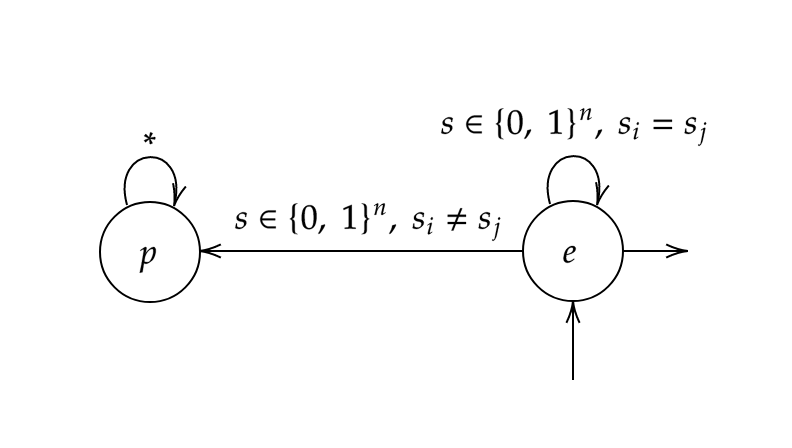
\includegraphics[scale=0.5]{auto_egalite.png}
    \caption{\label{Auto_Egalite} Automate pour la formule $x_i=x_j$}
  \end{figure}

  \begin{figure}[!h]
    \centering
    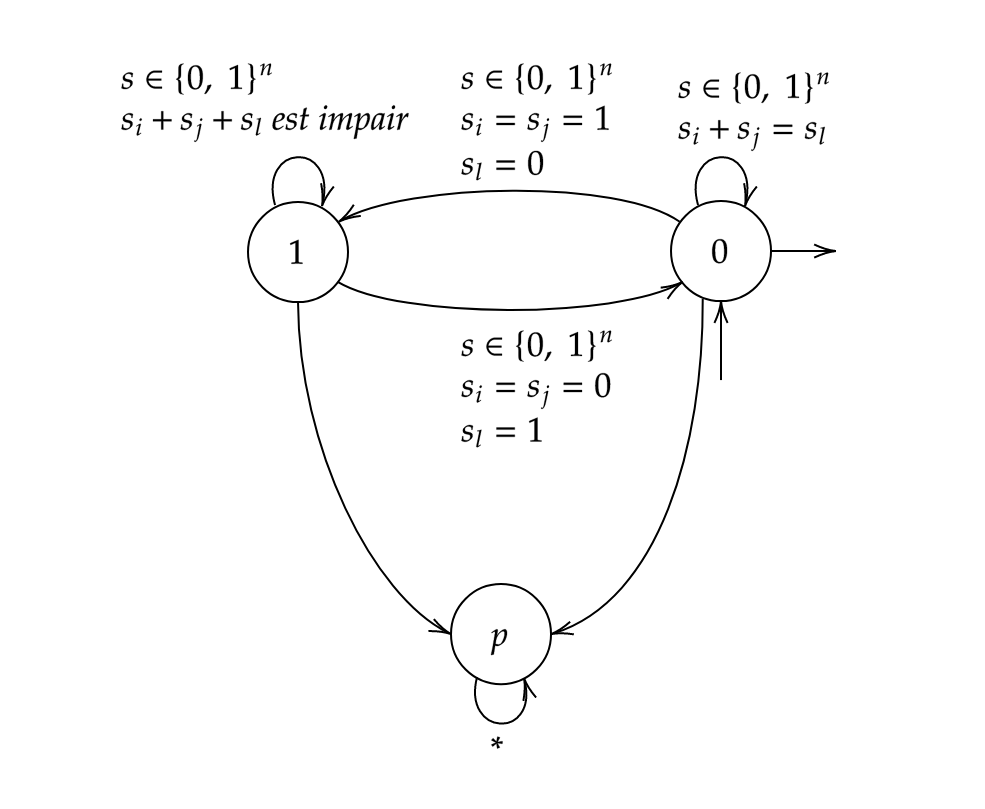
\includegraphics[scale=0.5]{auto_somme.png}
    \caption{\label{Auto_Egalite} Automate pour la formule $x_i+x_j=x_l$}
  \end{figure}

La construction formelle de $\mathcal{A}_{F_n}$ est un peu lourde, je ne la présente pas. Il est facile de comprendre que le langage de l'automate est bien $X_n$.

Nous allons maintenant construire $\mathcal{A}_{F_{k}}$ à partir de $\mathcal{A}_{F_{k+1}}$. On a $F_{k} = \#_k x_k, F_{k+1}$, on doit discuter du cas o\`u $\#_k$ est $\forall$ et $\#_k$ est $\exists$. On tra\^ite d'abord le cas du quantificateur existenciel.

On suppose que $F_k = \exists x_k, F_{k+1}$. Pour prendre en compte le quantificateur existenciel $\exists x_k$, il suffit d'``ingorer'' l'indice $k$ dans les transitions. Plus formellement, si $\mathcal{A}_{F_k}=(\{0, 1\}^k, Q, \delta, I, S)$ o\`u $Q$ est l'ensemble fini des états, $I\subseteq Q$ est l'ensemble des états initiaux, $S\subseteq Q$ est l'ensemble des états finaux et $\delta : \{0, 1\}^k \times Q \rightarrow Q$ est la fonction de transitions. Alors, on pose $\mathcal{A}_{F_k}=(\{0, 1\}^{k-1}, Q, \delta', I', S)$ avec $\delta'((d_1, \ldots, d_{k-1}), q') = q$ si et seulement si $\delta((d_1, \ldots, d_{k-1}, d_k), q') = q$ et $I' = I \cup \delta((0, \ldots, 0, *), I)$ l'ensemble des états accessibles à partir des états initiaux de $\mathcal{A}_{F_{k+1}}$ en lisant des $0$ sur les $k$ premières entrées.

Montrons que le langage reconnu par $\mathcal{A}_{F_k}$ est exactement les encodages en binaires avec potentiellement des vecteurs nuls devant des $k$-uplets d'entiers $(x_1, \ldots x_k)$ tels que $F_k(x_1, \ldots, x_k)$ est vraie. On sait que le langage de $\mathcal{A}_{F_{k+1}}$ est exactement les encodages des $k+1$-uplets d'entiers $(x_1, \ldots x_k, x_{k+1})$ tels que $F_{k+1}(x_1, \ldots, x_k, x_{k+1})$ est vraie. Soit $(x_1, \ldots x_k)$ tels que $F_k(x_1, \ldots, x_k)$ est vraie, alors s'il existe $x_{k+1} \in \mathbb{N}$ tel que $F_{k+1}(x_1, \ldots, x_{k+1})$ est vraie, c'est à dire qu'il existe un chemin d'un état initial à un état final dans lequel les $k$ premiers entiers qui indicent le chemin sont $(x_1, \ldots, x_k)$. Donc tout $k$-uplet encodé dans $X_k$ au moins un prolongement dans $X_{k+1}$. De plus, si $(x_1, \ldots, x_{k+1})$ indice un chemin d'un état initial de $\mathcal{A}_{F_{k+1}}$ à un état final, cela signifie qu'il existe $x_k \in \mathbb{N}$ tel que $F_{k+1}(x_1, \ldots, x_{k+1})$ est vraie et donc $F_k(x_1, \ldots, x_k)$ est vraie. Cela signifie que tous les encodages de $(x_1, \ldots, x_k)$ doivent \^etre dans $X_k$. On a bien le langage souhaité pour $\mathcal{A}_{F_k}$ grace à l'astuce d'ajouter des états initiaux.

On sait que l'on peut ré-écrire $F_{k}=\forall x_k, F_{k+1}$ en $F_{k}=\lnot \exists x_k, \lnot F_{k+1}$. Ainsi, traiter le cas du quantificateur existenciel permet de traiter le cas du quantificateur universel. En effet, si $L(\mathcal{A_{F_{k+1}}}) = X_{k+1}$ alors, le langage $\overline{X_{k+1}}$ est l'ensemble des encodages des tuples tels que $F_{k+1}$ n'est pas vraie (ie. $\lnot F_{k+1}$ est vraie), qui est reconnu par l'automate complémentaire à $\mathcal{A_{F_{k+1}}}$ (qui doit \^etre déterminisé et complété si ce n'est pas encore le cas). Ainsi, si l'on sait tra\^iter le cas existentiel et que l'on applique l'opération de complémentarisation à nouveau, on obtient un automate qui reconnait $X_k$.

On obtient ainsi un automate $\mathcal{A_{F}}$, nous allons ici conclure en disant que $L(\mathcal{A_{F}})$ est vide si et seuelement si $F$ est fausse dans $\mathbb{N}$. En remontant une étape de construction (il y a au moins un quantificateur), on obtient un automate dont le langage est $X_1$ et on observe que pour tout mot dans $X_1$, il existe un mot de m\^eme longueur dans $\mathcal{A_{F}}$. Et donc, il existe $x_1 \in \mathbb{N}$ tel que $F_1(x_1)$ est vraie alors si et seulement si $X_1$ est non vide, si et seulement si $L(\mathcal{A_{F}})$ et si et seulement si $F = \exists x_1, F_1(x_1)$ est vraie dans $\mathbb{N}$. Il est facile de décider algorithmiquement si un automate a un langage vide ou non, et donc, le problème donné est bien décidable.
\end{proof}

\end{document}

